\documentclass[11pt, oneside]{article}
\usepackage[utf8]{inputenc}                        % utf8
\usepackage[T1]{fontenc}                           % fix font encoding
\usepackage[english]{babel}                        % language
\usepackage{titling, geometry, hyperref, fancyhdr, algorithm}
\usepackage{amsmath, amssymb, amsthm}              % ams mathematical packages
\usepackage{physics, mathtools, bm}                % extra math packages
\usepackage{graphicx, subcaption, wrapfig}         % images
\usepackage{fvextra, textcomp, CJKutf8, ulem}      % misc. text formatting
\usepackage[autostyle, english=american]{csquotes} % quotes
\usepackage[shortlabels]{enumitem}                 % lists
\usepackage{tikz, pgfplots, tikz-network}          % plots and graphs
\usepackage[noend]{algpseudocode}                  % algorithm psuedocode
\usepackage[cache=true]{minted}                    % source code
\usepackage[style=ieee]{biblatex}                  % bibliography
\geometry{a4paper}

\pgfplotsset{compat=1.17}                          % version of pgfplots

\hypersetup{
  colorlinks=true,
  urlcolor=cyan,
  linkcolor=black
}

\setminted[]{
  linenos=false,
  breaklines=true,
  encoding=utf8,
  fontsize=\normalsize,
  frame=lines,
  framesep=2mm
}

% https://tex.stackexchange.com/questions/343494/minted-red-box-around-greek-characters
\makeatletter
\AtBeginEnvironment{minted}{\dontdofcolorbox}
\def\dontdofcolorbox{\renewcommand\fcolorbox[4][]{##4}}
\makeatother

\graphicspath{{./images/}}
\addbibresource{ref.bib}

\newcommand{\emphasis}[1]{\textbf{\textit{#1}}}
\newcommand{\dash}{\textquotesingle}

\title{One-Handed Tips and Tricks}
\author{Stephen Huan}
\date{\today}

\begin{document}
\maketitle
% \tableofcontents

\section{Introduction}

Miscellaneous one-handed (OH) tips and tricks developed over
3 years of practicing the event. Many of these tips are applicable to
two-handed solving (2H), but not all.
I practice the Cross-F2L-Oll-PLL (CFOP) method for OH and 2H,
but I would argue Roux method users have a definitive advantage in OH and
possibly 2H as well.
Some people, like Stanley Chapel, use CFOP for 2H and Roux for OH.
This seems difficult to do so I wouldn't recommend it, but it is possible.

\enquote{Ratio} refers to the ratio between 2H times and OH times, e.g.
if my PB 2H ao50 is 9.23 and my PB OH ao50 is 13.12, then I have a 2H : OH ratio
of 13.12/9.23 = 1.42. Typical ratio for CFOP solvers is 1.5, which lowers with
practice and degree of specialization in OH.
Roux solvers can reach a ratio as low as 1.2, e.g. Iuri Caravalho.

Notable CFOP method users:
\begin{itemize} 
  \item \href{https://www.worldcubeassociation.org/persons/2012PARK03}{Max Park}
    - Current OH world record (WR) average holder, specializes in NxN's. 
  \item \href{https://www.worldcubeassociation.org/persons/2009ZEMD01}{Feliks Zemdegs}
    - Generalist and one of the most famous cubers of all time.
  \item \href{https://www.worldcubeassociation.org/persons/2010CANT02}{Antoine Cantin}
    - OH specialist holding many former OH WRs. Has a useful
    \href{https://sites.google.com/site/antoineccantin/Home}{website}
    and \href{https://www.youtube.com/user/antoineccantin}{YouTube channel}.
\end{itemize}

Notable Roux method users:
\begin{itemize} 
  \item \href{https://www.worldcubeassociation.org/persons/2015MANS03}{Kian Mansour}
    - Former OH WR average holder, the only WR set with Roux as far as I know.
    Has a useful \href{https://sites.google.com/view/kianroux}{website} and
    \href{https://www.youtube.com/c/PenguinsDontFly/videos}{YouTube channel}.
  \item \href{https://www.worldcubeassociation.org/persons/2015CARV06}{Iuri Carvalho}
    - Fast Rouxer with a 1.2 ratio. 
  \item \href{https://www.worldcubeassociation.org/persons/2016CHAP04}{Stanley Chapel}
    - Generalist using CFOP for 2H and Roux for OH. 
\end{itemize}

The dominant difference between OH and 2H solving is that OH is much slower.
This gives you more time to think and do fancier things than you could do 2H.
For example, CFOP and Roux are arguably even for 2H solving, but Roux is nearly
objectively better for OH solving (if you can master M flicks).
The decreased move count wins over the increased thinking time, and the 2gen
<M, U> edge steps can be done surprisingly quickly.
For CFOP, the slower turn speed of OH makes difficult algsets and techniques
like ZBLL and psuedoslotting more viable.

\section{Tips \& Tricks}
\begin{itemize}
  \item Why do OH? As I said on the first page, it makes solving more
    intellectual since you have more time to think,
    (but also less intellectual, since OH times are more turning
    dependent than 2H times) and provides an alternative physical challenge.
    The main reason for me is just that it looks really cool.
  \item Which hand to use? I prefer left hand, since for a right-hand dominant
    solver most of your turns will be <R, U> when 2H solving. If you use your
    left hand for OH, you can use the same <R, U> algorithms. If you use your
    right hand, you have to mirror all your algorithms to <L, U>.
    The strength difference between a pinkie on the left hand and a pinkie
    on the right hand is probably minimal, and between staying in <R, U>
    and being able to still solve a cube if my dominant hand is injured,
    left hand wins out for me personally. Most top-level right handed cubers
    also use their left hand for OH.
  \item Color Neutrality (CN) is both easier and more important to do in OH
    than 2H. Since you have more thinking time, it's easier to find pairs.
    Cross (with its F moves) is a more difficult step (less ergonomic) on OH
    than in 2H, so a easier cross and 1-2 moves less with CN is worth it.
  \item Some people keep their other hand on the stackmat timer, so they can 
    stop very quickly. Kian Mansour has especially nice timer stops, as seen
    in his \href{https://www.youtube.com/watch?v=pCfLsh5vDt0}{former WR}.
    The benefit is obviously faster stops, but the drawback is an increased
    chance of DNF if you accidentally bump the other side.
    Personally, I don't use stackmats very often, so my right hand awkwardly
    hovers off to the side somewhere.
  \item Don't over warm-up before competing.
    The best results happen when your mind is warmed up
    but your hand warms up much faster than your mind (in like 5 solves).
    Since OH turning is very pinkie-ring finger dominant, it's easy to wear out
    just two fingers with a few solves. I can easily do > ao100's on 2H,
    but ao50's are usually too long for OH (my times inevitably trend up past
    25-30ish solves). What I like to do to warm up OH is to do 2H solves first,
    to warm up my mind, and then within 5ish OH solves that'll be
    peak performance.
  \item \enquote{Table abuse} refers to the action of using the table while
    solving. The table can be used as a \enquote{third hand} to maintain control
    while rotating or aligning layers. I personally never use the table, but
    Max Park's solves are very table dominant and Rouxers need the table to do
    <M, U> quickly. Since using the table is legal in WCA competitions, there's
    really no downside (except for the added time in picking up the cube and
    putting it down against the table repeatedly). It's something for you to
    integrate into your personal style accordingly. 
  \item Practice OH randomly, like on the bus \sout{or in class} or something.
    Since you only need one hand, and if you don't table,
    then you can do OH basically anywhere.
\end{itemize}

\section{Algorithms}
\begin{itemize}
  \item <R, U> is the best possible move set. Every other move is basically
    <R, U> with rotations so you want to stick with <R, U> as much as possible.
  \item A lot of OH turning is reducing the transition time between moves.
    If you're doing an R, make sure your index finger is in position to do the
    next U/U\dash. If you're doing a U, the opposite applies. Since the turning
    is slow, any unnecessary pauses have to be reduced.
  \item Do F with your thumb and F\dash\ with an index finger flick.
    They are surprisingly fast, and can be done with very little to no
    pinkie movement which speeds up transitions between moves. 
    Against popular wisdom I would argue F/F\dash\ are faster than D/D\dash\
    (which requires the entire hand to regrip for the 4th finger).
  \item Wide move are ok. r/r\dash are decent, but require shifting the pinkie
    over. r can sometimes be done with the 4th finger to remove that shift,
    if the pinkie is not in position to do r. In a similar vein, u\dash\ is ok,
    but requires a shift of the index finger downwards, but u is especially bad,
    since the movement from the standard position of the index finger from the
    BLU sticker to the FL edge is a giant jump. f' is nice because it can
    be done with the index finger flicking, for f it is hard to get the F layer
    to push up with the S layer because the thumb is on the F layer. 
  \item <M, U> can be really good but for CFOPers it's probably best to stick
    to <R, U>. The only PLL I do with <M, U> is H-perm, because the <R, U>
    variant is trash and all the M moves are M2's, so I don't have to do M's
    (M' and M2 can easily be done against a table, but M requires practice).
  \item Relearn PLLs
    \begin{itemize}
      \item Start with the EPLLs, Ua, Ub, and Z all have good <R, U> algorithms.
        H perm is more personal preference, but it does have a 2gen algorithm.
      \item I find E, Ra, and V perm worth learning alternative algorithms for.
        Of course, this depends on what algorithms you use for 2H.
    \end{itemize}
  \item Relearn OLLs
  \item Learn COLL (Corners of the last layer), an algset with 42 algorithms,
    but only 30 if sunes and anti-sunes are excluded (because they're so fast,
    people usually don't bother learning alternative sune/anti-sune).
    This algset allows you to solve corners at the same time as OLL, if all
    the edges are oriented (yellow cross on top). This means you're guaranteed
    to get an EPLL (Ua, Ub, H, Z) with a 1/12 chance of a PLL skip.
    Because EPLLs are ridiculously fast relative to normal PLLs,
    it is much more worthwhile to use COLL in OH than in 2H.
  \item Learn ZBLL, starting with 2GLL. ZBLL allows you to solve last layer with
    one algorithm if edges are oriented, and 2GLL is a subset of ZBLL where you
    only need <R, U> moves. There are 84 cases in total, but only 60 are worth
    learning. I used Antoine Cantin's
    \href{https://sites.google.com/site/antoineccantin/2gll}{website} for this.
    Keep in mind 2GLL and ZBLL recognition is much harder than COLL.
    The first level is recognizing OLL. Then, if you use corner data,
    you can do COLL. ZBLL is if you use edge data, adding another layer.

    On top of this, you have a 1/8 chance of edges being oriented, without
    edge control, and about a 1/6 chance for the case to be a 2GLL case.
    This is a 1/48 change overall, so you'd expected a 2GLL case every
    \textit{1 in 50 solves}. Compare this to OLL/PLL where not only are there
    less algorithms, you train a OLL/PLL every solve.
    You'd expect to take 20,000 solves before you see every single 2GLL once.

    Thus, learning 2GLL is very difficult compared to OLL/PLL/COLL and its
    benefits are pretty marginal. It's definitely more efficient to train other
    techniques first before learning 2GLL/ZBLL.
\end{itemize}

\section{Hardware}
\begin{itemize}
  \item Generally speaking, you'll want your OH cube faster and looser than your
    2H cube. This helps reduce finger strain and will improve your times.
    It is nice to have at least two cubes, and designate one for OH and the
    other for 2H so you can set them up differently.
    Use faster lubes for OH too (lube can drastically change my times). 
  \item Small (e.g. < 55mm) cubes don't really matter. 54mm is a nice size,
    even for 2H, but few cubes come in this form factor
    (GAN 354, DaYan GuHong v3). 50mm is too small.
    Personally, I use a MoYu mf3rs2m, which is a 56mm cube and my hands aren't
    particularity big. I would prefer 54mm if there was a good enough cube
    at that size, but it's not worth the performance sacrifices currently. 
  \item The Valk is a very popular cube for OH, and so is the MoYu Weilong WRM. 
  \item In general, good 2H cubes are usually good OH cubes, but you'll want to
    prioritize stability for OH (turning mistakes are more costly than in 2H).
  \item Some people use GAN cubes (e.g. Max Park, Feliks Zemdegs)
    but I personally can't get good times on them. The smooth feeling of GAN
    cubes leads to a lack of turning feedback, which is less ideal in OH.
\end{itemize}

% \printbibliography

\section{References}
\begin{enumerate}
  \item \href{https://www.worldcubeassociation.org/results/rankings/333oh/average}
    {World Cube Association (WCA) OH rankings}
  \item \href{https://www.youtube.com/watch?v=mUF3aPDTO-4}{J Perm's OH tutorial}
  \item \href{http://algdb.net/}{algdb}
\end{enumerate}

\begin{figure}[h!]
  \centering
  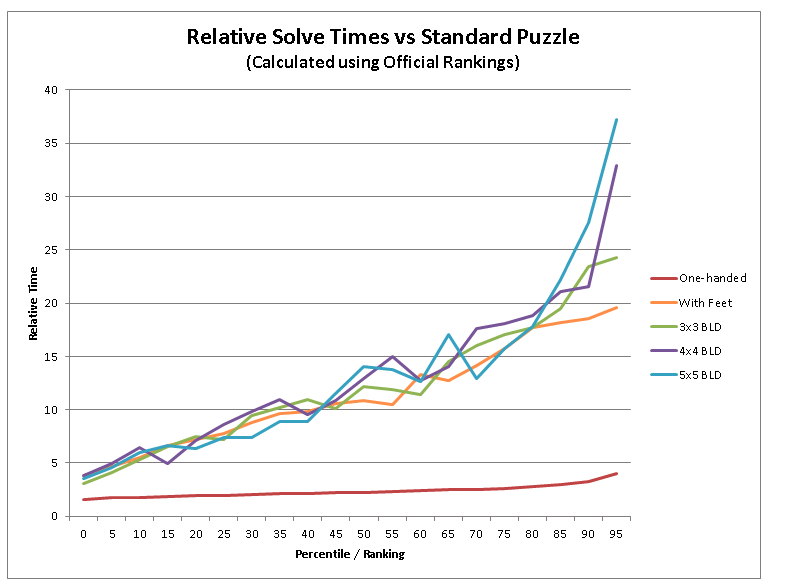
\includegraphics[scale=0.6]{ratio_graph}
  \caption{Ratio Graph of Side Events}
\end{figure}

\end{document}
